\documentclass[slidestop,compress,mathserif,c]{beamer}
\usepackage{listings}
\usepackage{color}
\usepackage{xcolor}
\usepackage{hyperref}
\definecolor{dkgreen}{rgb}{0,0.6,0}
\usepackage{fontspec,xunicode,xltxtra,beamerthemesplit}
%\usepackage{slashbox}
\usepackage{diagbox}
 \newfontfamily\times{Times New Roman}
%以下是各种演示主题,定义幻灯片中的所有细节
%\usetheme{default}
%\usetheme{Berlin}%这个主题比较好
%\usetheme{Pittsburgh}
%\usetheme{Rochester}
\usetheme{Berkeley}%这种演示主题比较好
%\usetheme{Goettingen}
%\usetheme{Hannover}
%\usetheme{Marburg}
%\usetheme{PaloAlto}%这种演示主题比较好
%\usetheme{Antibes}
%\usetheme{Darmstadt}
%\usetheme{JuanLesPins}
%\usetheme{Montpellier}
%\usetheme{Singapore}
%\usetheme{Boadilla}
%\usetheme{Madrid}
%\usetheme{AnnArbor}
%\usetheme{CambridgeUS}
%\usetheme{Copenhagen}
%\usetheme{Warsaw}

%以下是各种外部主题,确定幻灯的显示式样
%\useoutertheme{infolines}
%\useoutertheme{miniframes}
%\useoutertheme[height=0.1\textwidth,width=0.15\textwidth,hideothersubsections]{sidebar}
%\useoutertheme{smoothbars}
%\useoutertheme{split}
%\useoutertheme{shadow}
%\useoutertheme{tree}
%\useoutertheme{smoothtree}
%\useoutertheme[height=0.5\textwidth]{sidebar}

%以下是各种内部主题
%\useinnertheme{default}
%\useinnertheme{circles}
%\useinnertheme{rectangles}
\useinnertheme[shadow]{rounded}

%以下是各种颜色主题
%\usecolortheme{default}
%\usecolortheme{albatross}
%\usecolortheme{beaver}
%\usecolortheme{beetle}
%\usecolortheme{crane}
%\usecolortheme{dolphin}
%\usecolortheme{dove}
%\usecolortheme{fly}
%\usecolortheme{lily}
%\usecolortheme{orchid}
%\usecolortheme{rose}
%\usecolortheme{seagull}
\usecolortheme{seahorse}
%\usecolortheme{sidebartab}
%\usecolortheme{structure}
%\usecolortheme{whale}
%\usecolortheme{wolverine}

%以下是各种字体主题
%\usefonttheme{default}
%\usefonttheme[onlymath]{serif}
%\usefonttheme{structurebold}
%\usefonttheme{structureitalicserif}
%\usefonttheme{structuresmallcapsserif}
\newcommand{\tablecell}[2]{\begin{tabular}{@{}#1@{}}#2\end{tabular}}   % 表格内换行,用法\tablecell{c}{balabalba\\balabalba}
\setsansfont[Mapping=tex-text, BoldFont={微软雅黑 Bold}]{微软雅黑}

% 中文环境自动换行
\XeTeXlinebreaklocale "zh"  % 表示用中文的断行
\XeTeXlinebreakskip = 0pt plus 1pt % 多一点调整的空间

% 中文环境修正导航栏
\makeatletter
\setbeamertemplate{blocks}[rounded][shadow=true] 
\def\beamer@linkspace#1{
  \begin{pgfpicture}{0pt}{-1.5pt}{#1}{5.5pt}
    \pgfsetfillopacity{0}
    \pgftext[x=0pt,y=-1.5pt]{.}
    \pgftext[x=#1,y=5.5pt]{.}
  \end{pgfpicture}}
\makeatother

% 超链接高亮显示
\hypersetup{CJKbookmarks=true,
colorlinks=true,
citecolor=blue,
linkcolor=blue,
urlcolor=blue,
bookmarksopen=true,
breaklinks=true
}

% 幻灯片切换方式
%\transblindshorizontal 	% 水平百叶窗
%\transblindsvertical 		% 垂直百叶窗
%\transboxin				% 盒状收缩
%\transboxout				% 盒状展开
%\transdissolve				% 溶解
%\transglitter
%\transsplithorizontalin	% 上下向中央收缩
%\transsplitverticalin		% 垂直向中央收缩
%\transsplithorizontalout	% 上下向中央展开
%\transsplitverticalout		% 垂直向中央展开
%\transwipe					% 从下抽出


\title{最优化概述}
\author{Liu Zheng}
\date{\today}
\institute{同济大学电信学院}

\logo{\color{blue!50}\scalebox{2}{{
\includegraphics[height=0.8cm]{logo.jpg}\vspace{220pt}}}}

% 设定frametitle居中
\makeatletter 
\long\def\beamer@@frametitle[#1]#2{% 
  \beamer@ifempty{#2}{}{% 
    \gdef\insertframetitle{\centering{#2\ifnum\beamer@autobreakcount>0\relax{}\space\usebeamertemplate*{frametitle continuation}\fi}}% 
  \gdef\beamer@frametitle{#2}% 
  \gdef\beamer@shortframetitle{#1}% 
}% 
} 
\makeatother


\titlegraphic{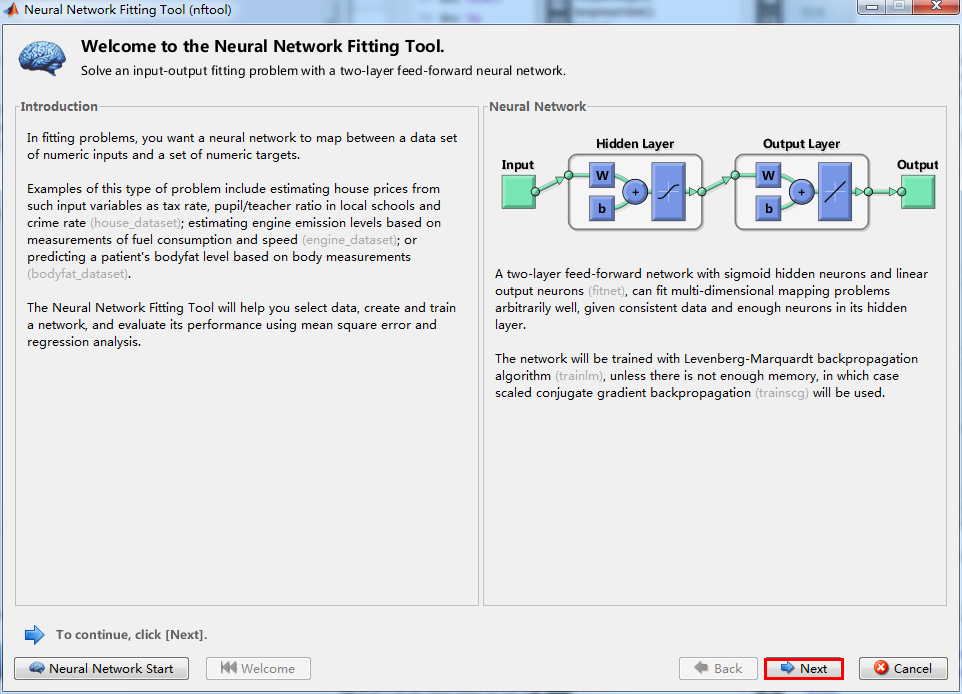
\includegraphics[width=2.3cm]{2.png}}
\begin{document}

\frame{\titlepage}

\section{最优化方法概述}


%%%%%%%%%% One Slide %%%%%%%%%%
%\subsection{\hfill }
\begin{frame}
\frametitle{概述}
\begin{itemize}
    \item 最优化理论和方法是近二十多年来发展十分迅速的一个数学分支
    \item 在数学上,最优化是一种求极值的方法
    \item 最优化已经广泛的渗透到工程、经济、电子技术等领域
\end{itemize}

\end{frame}
%%%%%%%%%% Slide End %%%%%%%%%%


%%%%%%%%%% One Slide %%%%%%%%%%
%\subsection{\hfill Overview}
\begin{frame}
\frametitle{概述}
\begin{itemize}
    \item 在实际生活中,人们做任何事情,不管是分析问题,还是进行决策,都要用一种标准衡量以下是否达到来最优。(比如基金人投资)
    \item 在各种科学问题、工程问题、生产管理、社会经济问题中,人们总是希望在有限的资源条件下,用尽可能小的代价,获得最大的收益。(比如保险)
\end{itemize}
\end{frame}
%%%%%%%%%% Slide End %%%%%%%%%%

%%%%%%%%%% One Slide %%%%%%%%%%
%\subsection{\hfill Overview}
\begin{frame}
\frametitle{几个概念}
\begin{itemize}
    \item 最优化是从所有可能方案中选择最合理的一种,以达到最优目标的学科
    \item 最优方案是达到最优目标的方案
    \item 最优化方法是搜寻最优方案的方法
    \item 最优化理论就是最优化方法的理论
\end{itemize}

\end{frame}
%%%%%%%%%% Slide End %%%%%%%%%%

%%%%%%%%%% One Slide %%%%%%%%%%
\subsection{\hfill 经典极值问题}
\begin{frame}
\frametitle{经典极值问题}
包括
\begin{itemize}
    \item 无约束极值问题
       $$ \min_xf(x) $$ 
    \item 约束条件下的极值问题
      \begin{eqnarray*}
        & \underset{x}{\min}f(x)\\
      s.t. & g_i(x)\leq 0, i=1,2,\cdots,m\\
           & h_i(x)=0, i=1,2,\cdots,n
  \end{eqnarray*}
  其中,极大值问题可以转换为极小值问题来进行求解。如求:
   $ \underset{x}{\max}f(x) $ 
  可以转换为: $ \underset{x}{\min}-f(x) $ 
\end{itemize}

\end{frame}
%%%%%%%%%% Slide End %%%%%%%%%%

%%%%%%%%%% One Slide %%%%%%%%%%
\subsection{\hfill 无约束极值问题}
\begin{frame}
\frametitle{无约束极值问题}
\begin{figure}[htbp]
  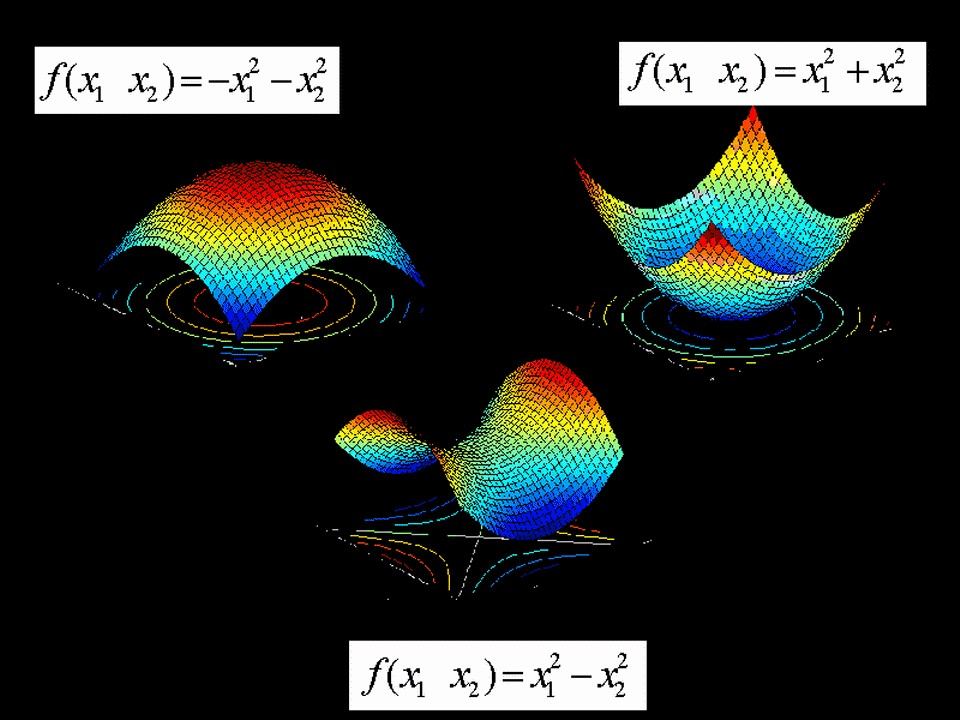
\includegraphics[height=7cm]{noneyueshu.jpg}
\end{figure}

\end{frame}
%%%%%%%%%% Slide End %%%%%%%%%%

%%%%%%%%%% One Slide %%%%%%%%%%
\subsection{\hfill 有约束最优化}
\begin{frame}
\frametitle{有约束最优化}
最优化方法分类
\begin{enumerate}[(1)~]
  \item \textcolor{red}{线性最优化}:目标函数和约束条件都是线性的则称为线性最优化。
    
    \textcolor{red}{非线性最优化}:目标函数和约束条件如果含有非线性的,则称为非线性最优化。
     
  \item \textcolor{red}{静态最优化}:如果可能的方案与时间无关,则是静态最优化问题。
        
    \textcolor{red}{动态最优化}:如果可能的方案与时间有关,则是动态最优化问题
\end{enumerate}

\end{frame}
%%%%%%%%%% Slide End %%%%%%%%%%

%%%%%%%%%% One Slide %%%%%%%%%%
\subsection{\hfill 有约束最优化问题的数学建模}
\begin{frame}
\frametitle{数学建模}
有约束最优化模型一般具有以下形式:
\begin{center}
\begin{tabular}{ccc}
  \tablecell{c}{ $ \underset{x}{\min}f(x) $ \\ $ s.t.~\cdots\cdots $ } & 或 & \tablecell{c}{ $ \underset{x}{\max}f(x) $ \\ $ s.t.~\cdots\cdots $ } 
\end{tabular}
\end{center}
其中 $ f(x) $ 为目标函数,省略号表示约束式子,可以是等式约束,也可以是不等式约束。
\end{frame}
%%%%%%%%%% Slide End %%%%%%%%%%

%%%%%%%%%% One Slide %%%%%%%%%%
\subsection{\hfill 最优化方法主要内容}
\begin{frame}
\frametitle{最优化方法主要内容}
根据目标函数,约束条件的特点将最优化方法包含的主要内容大致如下划分:
\begin{itemize}
\item 线性规划
\item 整数规划
\item 非线性规划
\item 智能优化方法
\item 变分法与动态规划
\end{itemize}
\end{frame}
%%%%%%%%%% Slide End %%%%%%%%%%


\section{线性规划与整数规划}
%%%%%%%%%% One Slide %%%%%%%%%%
%\subsection{\hfill Overview}
\begin{frame}
\frametitle{线性规划与整数规划}
~~~~在许多线性规划问题中,要求最优解必须取整数.例如
所求的解是机器的台数、人数车辆船只数等.如果所得的解
中决策变量为分数或小数则不符合实际问题的要求.

~~~~对于一个规划问题,如果要求全部决策变量都取整数,
称为纯(或全)整数规划;如果仅要求部分决策变量取整数,
称为混合整数规划问题.有的问题要求决策变量仅取0或1两
个值,称为0-1规划问题.

~~~~整数规划简称为IP问题(Integer Programming,IP)或ILP问题(Integer Linear Programming).这里主要讨论的是整数线性规划。

\end{frame}
%%%%%%%%%% Slide End %%%%%%%%%%

%%%%%%%%%% One Slide %%%%%%%%%%
\subsection{\hfill 整数规划}
\begin{frame}
\frametitle{整数规划}
\begin{itemize}
\item 最优化问题中的所有变量均为整数时,这类问题称为整数规划问题。
\item 如果线性规划中的所有变量均为整数时,称这类问题为线性整数规划问题。
\item 整数规划可分为线性整数规划和非线性整数规划 ,以及混合整数规划等。
\item 如果决策变量的取值要么为0,要么为1,则这样的规划问题称为0-1规划。
\end{itemize}
\end{frame}
%%%%%%%%%% Slide End %%%%%%%%%%

%%%%%%%%%% One Slide %%%%%%%%%%
%\subsection{\hfill Overview}
%\begin{frame}
%\frametitle{解}
%该工厂生产产品I  x1件,生产产品II  x2件,我们可建立如下数学模型:
%\begin{center}
%  \begin{eqnarray*}
%    \max z=2x_1+3x_2\\
%    s.t.\left\{
%    \begin{array}{lclcr}
%      x_1&+&2x_2&\leq&8\\
%      4x_1&&&\leq&16\\
%      &&4x_2&\leq&12\\
%      x_1&,&x_2&\geq&0
%    \end{array}\right.
%  \end{eqnarray*}
%\end{center}
%
%\end{frame}
%%%%%%%%%% Slide End %%%%%%%%%%

%%%%%%%%%%% One Slide %%%%%%%%%%
%%\subsection{\hfill }
%\begin{frame}
%\frametitle{一个简单的例子}
%要从甲城调出蔬菜2000吨,从乙城调出蔬菜2500吨,从丙地调出3000吨,分别供应A地2000吨,B地2300吨、C地1800吨、D地1400吨,已知每吨运费如下表:
%\begin{center}
%\begin{tabular}{|*5{c|}}
%  \hline
%  \backslashbox{调出单位}{供应单位}&A&B&C&D\\\hline
%  甲&21&27&13&40\\\hline
%  乙&45&51&37&20\\\hline
%  丙&32&35&20&30\\\hline
%
%\end{tabular}
%\end{center}
%问:如何调拨才能使运费最省? 
%\end{frame}
%%%%%%%%%%% Slide End %%%%%%%%%%
%
%
%
%%%%%%%%%%% One Slide %%%%%%%%%%
%%\subsection{\hfill }
%\begin{frame}
%  \frametitle{假设}
%①假设题目中所给运费已考虑各地间公里数;
%
%②只考虑运量和运费,不考虑车辆调拨等其它相关因素
%
%③不考虑车辆返空的费用(或:所给运费已包含车辆返空的费用)
%
%变量说明:
%
% $ x_{ij} $ :从第 $ i $  城运往第j地的蔬菜数量( $ i=1,2,3;j=1,2,3,4 $ )
%
% $ a_{ij} $ :从第 $ i $  城运往第 $ j $ 地的单位运费( $  i=1,2,3;j=1,2,3,4  $ )
%
% $ b_i $ :从第 $ i $  城调出的蔬菜总量 
%
% $ c_j $ :第 $ j $  地所需蔬菜总量 
%
%\end{frame}
%%%%%%%%%%% Slide End %%%%%%%%%%
%
%%%%%%%%%%% One Slide %%%%%%%%%%
%%\subsection{\hfill Overview}
%\begin{frame}
%\frametitle{可以建立如下模型}
%     $$ \max z=\sum_{i=1}^3\sum_{j=1}^4a_{ij}x_{ij} $$ 
%\begin{center}
%  \begin{eqnarray*}
%    s.t.\left\{
%    \begin{array}{cc}
%      \sum_{j=1}^4x_{ij}=b_i&(i=1,2,3)\\
%      \sum_{i=1}^3x_{ij}=c_j&(i=1,2,3,4)\\
%      \tablecell{c}{ $ x_{ij}\geq0 $ \\ $ x_{ij}\leq\min(b_i,c_i) $ }&(i=1,2,3;j=1,2,3,4)
%
%    \end{array}\right.
%  \end{eqnarray*}
%\end{center}
%
%
%\end{frame}
%%%%%%%%%%% Slide End %%%%%%%%%%


%%%%%%%%%% One Slide %%%%%%%%%%
%\subsection{\hfill Overview}
\begin{frame}
\frametitle{列子}
~~~~某钢厂两个炼钢炉同时各用一种方法炼钢。第一种炼法每炉用  $ a $  小时,第二种用  $ b $  小时(包括清炉时间)。假定这两种炼法,每炉出钢都是 $ k $ 公斤,而炼  $ 1 $  公斤钢的平均燃料费第一法为  $ m $  元,第二法为  $ n $  元。若要求在  $ c $  小时内炼钢公斤数不少于  $ d $  ,试列出燃料费最省的两种方法的分配方案的数学模型。

\end{frame}
%%%%%%%%%% Slide End %%%%%%%%%%


%%%%%%%%%% One Slide %%%%%%%%%%
%\subsection{\hfill Overview}
\begin{frame}
\frametitle{解法}
设用第一种炼法炼钢  $ x_1 $  炉,第二种炼钢  $ x_2 $  炉
 $$ \max z=k(mx+ny) $$ 
\begin{center}
  \begin{eqnarray*}
    s.t.\left\{
      \begin{array}{ccc}
        ax_1&\leq&c\\
        bx_2&\leq&c\\
        k(x_1+x_2)&\geq&d\\
        x_1,x_2&\geq&0 \mbox{且为整数}
    \end{array}\right.
    \end{eqnarray*}
  \end{center}
  具体求解运算在此不作过多叙述,都是矩阵运算,相信大家对纯公式推导演算没多大兴趣。
\end{frame}
%%%%%%%%%% Slide End %%%%%%%%%%


%%%%%%%%%% One Slide %%%%%%%%%%
%\subsection{\hfill 基本算法}
\subsection{\hfill 单纯形法}
\begin{frame}
\frametitle{单纯形法}
~~~~单纯形法是优美国数学家G.B.Dantzig提出的,该方法的基本出发点就是在可行域(凸集)的定点中搜索最优点。搜索的过程是一个迭代的过程。首先找到一个基本可行解,判别它是否为最优解,如不是就找一个更好的基本可行解,再进行判别。如此迭代,直至找到最优解,或者判定该问题无界。

\end{frame}
%%%%%%%%%% Slide End %%%%%%%%%%

%%%%%%%%%% One Slide %%%%%%%%%%
%\subsection{\hfill 凸集}
\begin{frame}
\frametitle{凸集}
定义: $ \mathbf{X} $ 是 $ \mathbf{E}^n $  空间的点集, $ x_1 $  和 $ x_2 $ 是 $ \mathbf{X} $ 上任意两点,若对任意 $ 0\leq\lambda\leq1 $ 使得 $$ \lambda x_1+(1-\lambda)x_2\in \mathbf{X} $$ 
则称 $ \mathbf{X} $ 为凸集。
\begin{center}
  \begin{figure}[htbp]
    \begin{minipage}{0.4\textwidth}
    \caption{凸集}
    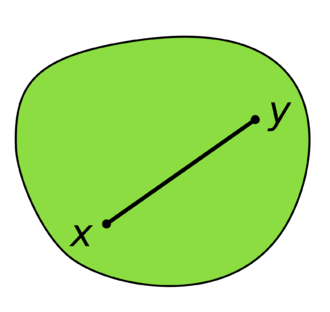
\includegraphics[width=3cm]{tuji.png}
  \end{minipage}
    \begin{minipage}{0.4\textwidth}
    \caption{非凸集}
    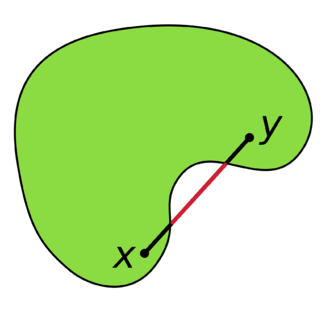
\includegraphics[width=3cm]{feituji.png}
  \end{minipage}
  \end{figure}
\end{center}
\end{frame}
%%%%%%%%%% Slide End %%%%%%%%%%

%%%%%%%%%% One Slide %%%%%%%%%%
\begin{frame}
\frametitle{单纯形法基本形式}
~~~~用单纯法求解时,常将标准形式化为:
\begin{eqnarray*}
  \begin{array}{cc}
  \min & f=cx\\
  s.t.&
    Ax=b\\
    &x\geq0
  \end{array}
\end{eqnarray*}
这里
\begin{center}
 $ A=(a_{ij})_{m,n} $ 

 $ x=(x_1,x_2,\cdots,x_n)^T $ 

 $ b=(b_1,b_2,\cdots,b_n)^T $ 

 $ c=(c_1,c_2,\cdots,c_n) $ 
\end{center}
\end{frame}
%%%%%%%%%% Slide End %%%%%%%%%%


%%%%%%%%%% One Slide %%%%%%%%%%
%\subsection{\hfill Overview}
\begin{frame}
\frametitle{解法}
一般步骤如下:

(1)寻找一个初始的基本可行解。

(2)检查现行的基本可行解是否最优,如果为最优,
则停止迭代,已找到最优解,否则下一步。

(3)移至目标函数值有所改善的另一个基本可行解,
然后转回到步骤(2)。
\\[1cm]

~~~~~~算法思路如上,具体迭代、矩阵运算过于数学化,在此不作展开。
\end{frame}
%%%%%%%%%% Slide End %%%%%%%%%%


%%%%%%%%%%% One Slide %%%%%%%%%%
%%\subsection{\hfill Overview}
%\begin{frame}
%  \frametitle{确定初始的基本可行解}
%
%  ~~~~~~确定初始的基本可行解等价于确定初始的可行基,一旦初始的可行基确定了,那么对应的初始基本可行解也就唯一确定
%
%  ~~~~~~为了讨论方便,不妨假设在标准型线性规划中,系数矩阵 $ A $ 中前 $ m $ 个系数列向量恰好构成一个可行基,即
%   $ A=(BN) $ ,
%  
% ~~~~~~ 其中
%   $ B=(P_1,P_2,\cdots,P_m) $ 为基变量 $ x_1,x_2,\cdots,x_m $ 的系数列向量构成的可行基,
%  $ N=(p_{m+1},P_{m+2},\cdots,P_n) $ 为非基变量  $ x_{m+1},x_{m+2},\cdots,x_n $  的系数列向量构成的矩阵。 
%
%\end{frame}
%%%%%%%%%%% Slide End %%%%%%%%%%


%%%%%%%%%% One Slide %%%%%%%%%%
\subsection{\hfill 多目标规划}
\begin{frame}
\frametitle{多目标规划}
~~~~~~多目标规划法也是运筹学中的一个重要分支,它是在线性规划的基础上,为解决多目标决策问题而发展起来的一种科学管理的数学方法

~~~~~~多目标规划的概念是 1961年由美国数学家查尔斯和库柏首先提出的。
\end{frame}
%%%%%%%%%% Slide End %%%%%%%%%%

%%%%%%%%%% One Slide %%%%%%%%%%
%\subsection{\hfill Overview}
\begin{frame}
\frametitle{多目标规划标准型}
求  $ \mathbf{x}={x_1,x_2,\cdots,x_n}\in D\subset E^n $ ,使
      \begin{eqnarray*}
        & \min \mathbf{f}(x)=\{f_1(x),f_2(x),\cdots,f_N(x)\}\\
      s.t. & h_l(\mathbf{x})= 0, l=1,2,\cdots,L\\
           & g_m(\mathbf{x})\leq0, m=1,2,\cdots,M
  \end{eqnarray*}
式中, $ n $  为自变量 $ \mathbf{x} $ 的维数; $ L $ 为等式约束的数目; $ M $ 为不等式约束的数目
\end{frame}
%%%%%%%%%% Slide End %%%%%%%%%%


\section{非线性规划}
%%%%%%%%%% One Slide %%%%%%%%%%
%\subsection{\hfill Overview}
\begin{frame}
\frametitle{非线性规划问题的一般数学模型}
 $$ \min f(x) $$ 
\begin{eqnarray*}
  s.t.\begin{array}{ccc}
    g_i(x)&\leq&0,i=1,2,\cdots,m\\
    h_j(x)&=&0,j=1,2,\cdots,l
  \end{array}
\end{eqnarray*}
其中, $ x\in E^n $ , $ f(x) $ 为目标函数, $ g_i(x),h_j(x) $ 为约束函数,这些函数中至少有一个是非线性函数。

\end{frame}
%%%%%%%%%% Slide End %%%%%%%%%%


%%%%%%%%%% One Slide %%%%%%%%%%
\subsection{\hfill 凸函数}
\begin{frame}
\frametitle{凸函数}
定义:在某个开区间 $ C $ 内的凸函数 $ f $ 在 $ C $ 内连续,且在除可数个点之外的所有点可微。如果 $ C $ 是闭区间,那么 $ f $ 有可能在 $ C $ 的端点不连续。
  \begin{figure}[htbp]
    \centering
    \caption{凸函数}
    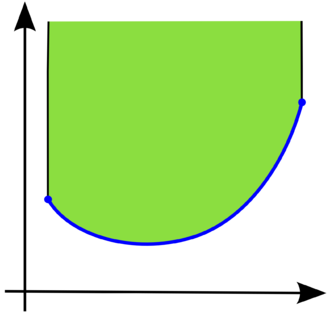
\includegraphics[width=3.7cm]{tuhanshu.png}
  \end{figure}
~~~~~~函数(蓝色)是凸的,当且仅当其上方的区域(绿色)是一个凸集。

\end{frame}
%%%%%%%%%% Slide End %%%%%%%%%%


%%%%%%%%%% One Slide %%%%%%%%%%
\subsection{\hfill 下降迭代法}
\begin{frame}
\frametitle{下降迭代法的基本思想}
~~~~~~任取一个初始迭代点
 $ \mathbf{x}^{(0)} $ ,在
 $ \mathbf{x}^{(0)} $ 处找一个下降方向
 $ \mathbf{p}^{(0)} $ ,移动
 $ \mathbf{x}^{(0)} $ 到
 $ \mathbf{x}^{(0)}+\lambda_0\mathbf{p}^{(0)} $ 处,令
 $ \mathbf{x}^{(1)}=\mathbf{x}^{(0)}+\lambda_0\mathbf{p}^{(0)} $ ,显然
 $ f(\mathbf{x}^{(1)})<f(\mathbf{x}^{(0)}) $ 。然后判断
 $ \mathbf{x}^{(0)} $ 是否为极小值点,若是,则停止迭代;否则,再从
 $ \mathbf{x}^{(1)} $ 出发,找比
 $ \mathbf{x}^{(1)} $ 更好的点
 $ \mathbf{x}^{(2)},\cdots, $ 如此继续,就产生了一个解点的序列
 $ \{\mathbf{x}^{(k)}\} $ ,满足

 $$ f(\mathbf{x}^{(0)})>f(\mathbf{x}^{(1)})>\cdots>f(\mathbf{x}^{(k)})>\cdots $$ 

\end{frame}
%%%%%%%%%% Slide End %%%%%%%%%%

\section{变分法与动态规划}

%%%%%%%%%% One Slide %%%%%%%%%%
%\subsection{\hfill Overview}
\begin{frame}
\frametitle{变分法和动态规划}
~~~~~~变分法涉及泛函,泛函又基于实变,以我的数学功底暂时无法完全理解,曾经在为专业课《工程光学》里提到过一次变分

原文为:

~~~~~~费马原理指出,光线从A点传到B点,经过任意多次的折射或反射,其光程为极值(极大值或极小值),可以用光程的一次变分为零来表示,即:
 $$ \delta\Delta=\delta\int_{A\to B}n(x,y,z)ds=0 $$ 

~~~~~~动态规划就不用多赘述了,

\end{frame}
%%%%%%%%%% Slide End %%%%%%%%%%




%%%%%%%%%% One Slide %%%%%%%%%%
\subsection{\hfill 动态规划}
\begin{frame}
  \frametitle{斐波那契数列(Fibonacci polynomial)}
  function fib(n)

~~~~if n = 0 or n = 1

~~~~~~~~ return 1

~~~~    return fib(n − 1) + fib(n − 2)

当n=5时,fib(5)的计算过程如下:
\begin{enumerate}
\item fib(5)
\item fib(4) + fib(3)
\item (fib(3) + fib(2)) + (fib(2) + fib(1))
\item ((fib(2) + fib(1)) + (fib(1) + fib(0))) + ((fib(1) + fib(0)) + fib(1))
\item (((fib(1) + fib(0)) + fib(1)) + (fib(1) + fib(0))) + ((fib(1) + fib(0)) + fib(1))
\end{enumerate}
\end{frame}
%%%%%%%%%% Slide End %%%%%%%%%%

%%%%%%%%%% One Slide %%%%%%%%%%
%\subsection{\hfill Overview}
\begin{frame}
  \frametitle{$O(n)$}
array map [0\ldots n] = { 0 => 0, 1 => 1  }

fib( n  )

~~~~if ( map m does not contain key n )

~~~~~~~~m[n] := fib(n − 1) + fib(n − 2)

~~~~~~~~~~~~return m[n]

~~~~~~将前$n$个已经算出的数保存在数组map中,这样在后面的计算中可以直接应用前面的结果,从而避免了重复计算。算法的运算时间变为$O(n)$
\end{frame}
%%%%%%%%%% Slide End %%%%%%%%%%

\section{智能优化方法}

%%%%%%%%%% One Slide %%%%%%%%%%
%\subsection{\hfill Overview}
\begin{frame}
  \frametitle{智能优化方法}
  \begin{itemize}
      \item 神经网络
      \item 模拟退火
      \item 遗传算法
      \item 蚁群算法
  \end{itemize}

\end{frame}
%%%%%%%%%% Slide End %%%%%%%%%%


%%%%%%%%%% One Slide %%%%%%%%%%
%\subsection{\hfill Overview}
\begin{frame}
\frametitle{Overview}


\end{frame}
%%%%%%%%%% Slide End %%%%%%%%%%


\end{document}
